\chapter{Modules}
\label{chap:Modules}

The source code of RespVis is structured into modules written in the ES module format.
Currently, all these modules are combined into a single, monolithic library bundle during the build process.
In the future, each module will be released on its own to allow users to import only the ones they need.
The reason for this is that most users will likely only require a subset of all the features included in the library and it would unnecessarily increase the size of their bundles to import all of them.
A good example of this is D3, which also separates its considerable amount of features into different modules that can be successively added to a project when the need arises.

At the time of writing, the RespVis library contains five different modules: the core, legend, tooltip, bar, and point modules.
Each of these modules contains submodules that have been grouped by thematic similarity.
The core module holds the core functionality of the library that all other modules depend on, which includes the layouter, axes, chart and chart window base components, and various utility functions and types.
The legend module contains the implementation of a legend component that is mostly meant to describe discrete data dimensions by rendering distinct values as labeled symbols.
The tooltip module holds functions to control the showing, placement, and content of tooltips, as well as utility functions that simplify the configuration and initialization of tooltips on series components.
% None of the modules listed so far contain components that render visual marks, which are characteristic for visualizations.
The bar module distinguishes between normal, grouped, and stacked bars and includes various low-level and high-level components to render each of those types.
Similarly, the point module contains low-level and high-level components to visualize point charts.
All of the different modules and the dependencies between them are shown in Figure~\ref{fig:Modules}.

\begin{figure}[tp]
  \centering
  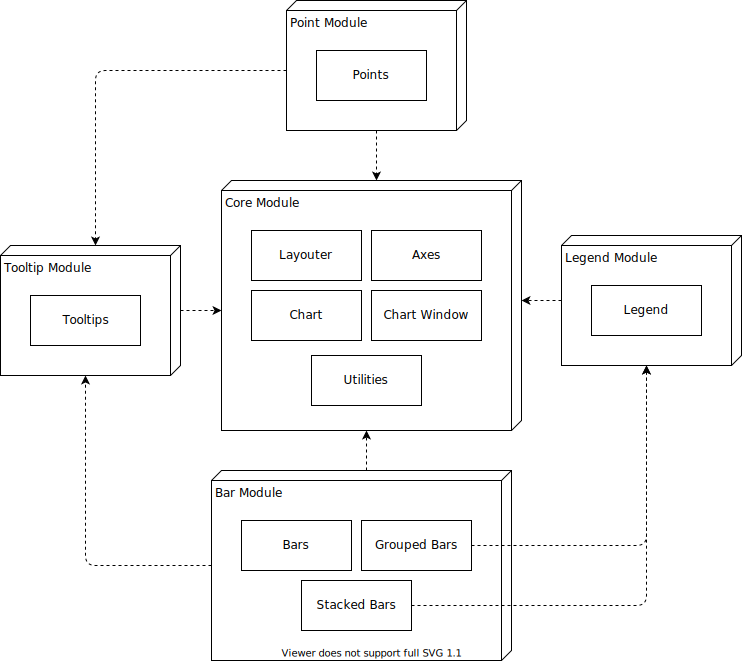
\includegraphics[keepaspectratio,width=\linewidth,height=\fullh]{diagrams/respvis-modules.pdf}
  \caption[Modules of RespVis]{
    This diagram shows the different modules of the RespVis library.
    It also shows the most important submodules contained in the individual modules.
    The directional arrows connecting modules indicate dependencies between them.
    \imgcredit{Image created by the author of this thesis using \href{https://www.diagrams.net/}{diagrams.net}.}
  }
  \label{fig:Modules}
\end{figure}


\section{Core Module}

The core module contains the necessary core functionality of the library.
It is the base module that all other modules depend on and includes various utility functions, the layouter, axes, chart base components, and chart window base components.
RespVis heavily relies on utility functions to reuse and structure recurring operations.
The core module contains utilities to deal with arrays, elements, selections, and texts, as well as geometric utilities that simplify the handling of positions, sizes, rectangles, circles, and paths.
The layouter is a custom component that enables controlling the layout of SVG elements with CSS.
% It achieves this by replicating the DOM tree of SVG elements that should be layed out with HTML \code{<div>} elements, applying the appropriate CSS configuration on the replicated elements, and storing their calculated layout information on the original SVG elements.
% Render functions can then use the stored layout information on layed out SVG elements to render their content so that it fits within the corresponding boundaries. 
Axis components have been included in the core module because they are important components that occur in nearly every visualization.
% However, since only cartesian charts have been implemented thus far, only cartesian axes can be found in the implementation.
Lastly, the chart and chart window components provide base functionalities that simplify the creation of more specialized charts and chart windows.
The core module implementation is located in the \code{src/lib/core/} directory of the project.

\subsection{Utilities}

The utilities provided by RespVis are split on multiple modules that are placed in the \code{utilities/} directory of the core module.
These modules include types and functions that perform array, element, selection and text operations as well as modules that simplify geometric operations with positions, sizes, rectangles, circles and paths.
Utility functions are grouped into modules by the type of entity they operate on.
This grouping is also reflected in the names of functions, which all begin with the type of entity a function is associated with.

\TODO{Capitalize "core module", "array utility module", ... ?}
Array utilities can be found in the \code{utilities/array.ts} module.
The \code{Array} class in the JavaScript base implementation already offers a wide variety of convenient methods to work with arrays.
These methods form a solid foundation that allows handling of a broad range of situations.
However, not everything is covered out of the box and some things require manual implementations, which is why the RespVis library offers additional functions that simplify commonly encountered tasks.
The \code{arrayEquals} function is used to verify equality of two arrays and also works if they contain nested arrays within them.
Type guard functions are used to determine the type of a variable at runtime.
For this purpose, two different array type guard functions are provided in the array utility module: \code{arrayIs}, which evaluates to true if the passed parameter is an array, and \code{arrayIs2D}, which evaluates to true if the passed parameter is a two-dimensional array.
The \code{arrayIs} function is merely a wrapper around the \code{Array.isArray} method.
Theoretically, the \code{Array.isArray} method could be used directly instead of the \code{arrayIs} function, but because the \code{arrayIs2D} function is required, the \code{arrayIs} function has also been added for consistency reasons.
The last function in the array utility module is the \code{arrayPartition} function.
This function receives an array and a partition size as parameters and returns a partitioned version of the input array with each chunk containing the number of items specified by the partition size parameter.


% elementRelativeBounds
% elementComputedStyleWithoutDefaults
% elementSVGPresentationAttrs

The element utilities module located at \code{utilities/elements.ts} in the core module contains functions and constants related to document elements.
The \code{elementRelativeBounds} function is used to calculate the bounding box of an element relative to the bounding box of its parent in viewport coordinates.
Internally, it uses the \code{getBoundingClientRect} function, which returns the actual bounding box of an element in viewport coordinates and, as opposed to other ways of accessing an element's position, it also takes transformations into account.
Every element has a set of CSS styles applied on them and the \code{Window.getComputedStyle} method can be used to access the active style of an element.
The style declaration object returned by this method contains all possible CSS properties and their values, regardless of whether or not they are set to default values.
Sometimes this behavior may be desired, but in this library, the computed style is used during the preparation of a downloadable SVG document to transform styles set in CSS to attributes on the individual elements.
If every possible style property on every element would be mapped to an attribute, the resulting SVG document would be unnecessarily bloated because only those properties that are not set to their default values actually have an effect.
For this reason, the \code{elementComputedStyleWithoutDefaults} function has been implemented to calculate the computed style of an element and remove all properties that are set to default values from the returned style declaration object.
This is implemented by adding a \code{<style-dummy>} element as a sibling of the element of interest, getting the computed styles of both elements, and calculating the difference between them.
To speed up these calculations, the \code{elementComputedStyleWithoutDefaults} function accepts an array of property names as its second parameter and will only consider the properties listed in this array.
The constant \code{elementSVGPresentationAttrs} array contains all names of the presentation attributes listed in the SVG 1.1 specification \parencite{SVG11}.
Since only these SVG attributes can be styled via CSS, only these properties need to be taken into account when preparing downloadable SVG documents.

% Transition default type variables
% Selection default type variables
% SelectionOrTransition default type variables
% Selection.attr add possible null return value
% Selection.dispatch allow Partial parameters
% isSelection
% isTransition

\TODO{When to write \code{Selection} and when to write Selection? What about plural? \code{Selections} or \code{Selection}s?}
Selection utilities are implemented in the \code{utilities/selection.ts} module.
They include typing improvements for the D3 \code{Selection}, \code{Transition}, and \code{SelectionOrTransition} interfaces and type guards to distinguish between \code{Selection}s and \code{Transition}s.
The \code{Selection}, \code{Transition}, and \code{SelectionOrTransition} interfaces allow the specification of four different type variables: the type of elements contained in the \code{Selection} or \code{Transition}, the type of data that is bound to those elements, the type of the parents of those elements, and the type of data that is bound to those parents.
In most cases, the type variables related to parent elements do not influence the logic of code using these interfaces and could be omitted to keep it more concise.
For this reason, these interface have been reexported with default types set on all of the type variables.
This means that whenever type variables need to be manually specified, only those that need to be set to specific types need to be explicitly stated.
Further typing improvements have been made to the \code{attr} and \code{dispatch} methods of the \code{Selection} interface.
The D3 type declarations of the \code{Selection.attr} method do not include \code{null} as a possible return value.
This is wrong because this method will actually result in a \code{null} value when reading an attribute that does not exist.
To fix this inconsistency and catch potential bugs related to this during compilation, the type declaration of the \code{Selection.attr} method has been overwritten in the Selection utility module to also include \code{null} as a possible return value.
A less important but nonetheless convenient improvement has been made to the type declaration of the \code{Selection.dispatch} method.
This method allows the dispatching of custom events with certain parameters that control different aspects of how this event is dispatched and the data that may be bound to it.
In practice, not all parameters need to be specified at every invocation because the implementation of the \code{Selection.dispatch} method will provide default values for all of them.
However, this is not reflected in the type declaration of the function, which requires every parameter to be provided every time the function is called.
To fix this, the Selection utility module provides a type declaration overwrite for the \code{Selection.dispatch} function that wraps the type of the parameters parameter into the \code{Partial} type.
Apart from these typing improvements, this module also provides the \code{isSelection} and \code{isTransition} type guard functions that are used to distiguish between \code{Selection}s and \code{Transition}s.


Utilities for dealing with \code{<text>} elements can be found in the \code{utilities/text.ts} module.
It contains rather basic functionalities that simply set specific data attributes to specific values on \code{<text>} elements.
The text utility module holds functions that set data attributes controlling the horizontal and vertical alignment of \code{<text>} elements, as well as their orientation.
Horizontal and vertical alignment is configured using the \code{textAlignHorizontal} and \code{textAlignVertical} functions.
These functions respectively set the \code{data-align-h} and \code{data-align-v} attribute on a Selection or Transition to the value passed into either function as a string enum parameter of type \code{HorizontalAlignment} or \code{VerticalAlignment}.
The \code{HorizontalAlignment} enum represents the string values \code{\"left\"}, \code{\"center\"} and \code{\"right\"}, while the \code{VerticalAlignment} enum represents the values \code{\"top\"}, \code{\"center\"} and \code{\"bottom\"}.
The distinct \code{data-align-h} and \code{data-align-v} attribute values are then used in the \code{respvis.css} file to declare different \code{text-anchor} and \code{dominant-baseline} values that control the alignment of \code{<text>} elements.
Text orientation is set using the \code{textOrientation} function.
This function sets the \code{data-orientation} attribute on a Selection or Transition to the value specified via the string enum parameter of type \code{Orientation}.
The \code{Orientation} enum represents the values \code{\"horizontal\"} and \code{\"vertical\"}.
These \code{data-orientation} attribute values are then used in CSS to set the \code{text-anchor}, \code{dominant-baseline}, and \code{transform} properties of a \code{<text>} element, in order to rotate it accordingly and position it correctly inside the bounding box calculated by the layouter.


% Position interface
% positionRound
% positionEquals
% positionToString
% positionFromString
% positionToAttrs (SelOrTrans)
% positionFromAttrs (SelOrTrans)
% positionToTransformAttr (SelOrTrans)

The core module also contains utilities that simplify geometric operations.
One of these utilities is the position utility module located at \code{utilities/position.ts}.
This module contains the \code{Position} interface and various functions to perform operations related to it.
The \code{Position} interface consists of the \code{x} and \code{y} number members.
Rounding these members is necessary to be able to correctly compare equality of two \code{Position}s and to not render unnecessarily long strings when transforming them into string representations.
This rounding is performed with the \code{positionRound} function, which allows the specification of the number of decimals the members variables should be rounded to.
Equality comparision between two \code{Position} variables can be performed with the \code{positionEquals} function, which evaluates to \code{true} if both \code{Position}s are equal and \code{false} if not.
To transform a \code{Position} into its string representation of the form \code{\"x, y\"}, the \code{positionToString} function can be used.
Its counterpart, the \code{positionFromString} function, can be used to transform a string in the correct format into a \code{Position}.
A large part of RespVis consists of modifying the attributes of elements.
Therefore, the \code{positionToAttrs} function can be used to set the \code{x} and \code{y} attributes of a \code{SelectionOrTransition} to the values of the \code{x} and \code{y} members of a \code{Position}.
Similarly, the \code{positionToTransformAttr} function can be used to set the \code{transform} attribute of a \code{SelectionOrTransition} to a translation representing a \code{Position}.
The position utility module also contains the \code{positionFromAttrs} function, which can be used to create a \code{Position} from the \code{x} and \code{y} attributes of a \code{SelectionOrTransition}.

% Size
% sizeRound
% sizeEquals
% sizeToString
% sizeFromString
% sizeToAttrs
% sizeFromAttrs

The size utility module is located at \code{utilities/size.ts} in the core module is very similar to the position utility module.
It contains the \code{Size} interface, which consists of the \code{width} and \code{height} number member variables.
The \code{sizeRound} function is used to round the member variables of a \code{Size} object to a certain number of decimals.
To compare two \code{Size} objects for equality, the \code{sizeEquals} function can be used.
Similar to the equivalent functions in the position utility module, the \code{sizeToString} and \code{sizeFromString} functions can be used to convert between \code{Size} objects and their string representations.
Moreover, the \code{sizeToAttrs} can be used to set the \code{width} and \code{height} attributes of a \code{SelectionOrTransition} to the values of a \code{Position} object and the \code{sizeFromAttrs} function can be used to create a new \code{Position} object from the values of these attributes.

% Rect
% rectRound
% rectEquals
% rectToString
% rectFromString
% rectToAttrs
% rectMinimized
% rectFitStroke
% rectPosition
% rectCenter
% rectLeft, rectRight, rectTop, rectBottom
% rectTopLeft, rectTopRight, rightBottomRight, rightBottomLeft

Utilities for dealing with rectangles can be found in the rectangle utility module, which is located under \code{utilities/rect.ts} in the core module.
This module contains the \code{Rect} interface, which is the union of the \code{Position} and \code{Size} interfaces and therefore describes an object with the number member variables \code{x}, \code{y}, \code{width}, and \code{height}.
Similar to the position and size utility modules, this module contains the \code{rectRound} function to round \code{Rect} objects, the \code{rectEquals} function to compare two of them for equality, the \code{rectToString} and \code{rectFromString} functions to convert between \code{Rect} objects and their string representations, and the \code{rectToAttrs} and \code{rectFromAttrs} functions to convert between objects and \code{x}, \code{y}, \code{width}, and \code{height} attributes.
Since the \code{Rect} interface is a combination of the \code{Position} and \code{Size} interfaces, most of the functions in this module internally use the functions provided by the position and size utility modules.
The \code{rectMinimized} function is used in transitions that grow or shrink a \code{<rect>} element from or to their center.
It creates a minimized version of the passed \code{Rect}, which is infinitely small and positioned at the original \code{Rect}'s center.
When declaring a stroke for SVG elements, it is drawn exactly on the outline of an element's silhouette.
This means that a stroke will extend outside the original bounds of an element by half the stroke width, which can lead to unwanted artefacts like the stroke of bars in a bar chart overlapping over the chart's axes.
To counteract this, the \code{rectFitStroke} function is provided to adjust the bounding box of \code{Rect} objects to account for a stroke of a certain width around them.
Lastly, the rectangle utility module provides functions to calculate specific positions inside of rectangles.
The most generic of these functions is the \code{rectPosition} functions.
This function enables the calculation of a position inside of a rectangle via a two-dimensional parameter that expresses a position as the percental width and height distance from a rectangle's top-left corner.
All other position-calculating rectangle utility functions are simply shorthand functions that internally call the \code{rectPosition} function.
The \code{rectCenter} function returns a \code{Position} object representing the center position of a \code{Rect} object.
The \code{rectLeft}, \code{rectRight}, \code{rectTop}, and \code{rectBottom} functions return \code{Position} objects that represent the middle position of a \code{Rect} object's edges.
Similarly, The \code{rectTopLeft}, \code{rectTopRight}, \code{rectBottomRight}, \code{rectBottomLeft} functions can be used to calculate the corner positions of a rectangle.

% Circle
% circleRound
% circleEquals
% circleToString
% circleFromString
% circleToAttrs
% circleFromAttrs
% circleMinimized
% circleFitStroke
% circlePosition
% circleInsideRect
% circleOutsideRect

The last geometric primitive whose handling is simplified by a RespVis utility module is a circle.
The circle utility module can be found at \code{utilities/circle.ts} in the core module.
It contains the \code{Circle} interface, which describes a circle object as a \code{center} property of type \code{Position} and a \code{radius} property of type \code{number}.
This module also contains equivalent functions to those found in previously mentioned utility modules: \code{circleRound}, \code{circleEquals}, \code{circleToString}, \code{circleFromString}, \code{circleToAttrs}, \code{circleFromAttrs}, \code{circleMinimized}, and \code{circleFitStroke}.
Furthermore, the \code{circlePosition} function can be used to calculate positions using an angle that defines the direction and an optional parameter that defines the distance from the circle's center as a percentage of the circle's radius.
The circle utility module also contains functions to create circles from rectangles.
These functions are the \code{circleInsideRect} function to calculate the largest circle that can fit inside of a rectangle and the \code{circleOutsideRect} function to calculate the smallest circle that encloses a rectangle.

% pathRect
% pathCircle

The purpose of the path utility module is to provide functions that simplify the creation of path definitions that can be set on \code{<path>} elements.
It is located at \code{utilities/path.ts} in the core module and only contains a small number of functions.
The \code{pathRect} function creates a path definition that represents a rectangle. 
A \code{<path>} element with a path definition representing a rectangle can be used instead of a \code{<rect>} element. 
Similarly, the \code{pathCircle} function creates a path definition that represents a circle.
Such a path definition is used on a \code{<path>} element to render a circle instead of using a \code{<circle>} element.
The reason for using \code{<path>} elements rather than more descriptive shape elements is that path elements can change their shape dynamically without replacing elements.
Since only the \code{d} attribute of a path needs to change when the path's shape is altered, it is also possible to smoothly transition between shapes by interpolating the path definition strings.

\subsection{Layouter}

% layouter

\subsection{Axes}

% base
% bottom axis
% left axis

\subsection{Chart}

% chart
% chart cartesian

\subsection{Chart Window}

% chart window
% menu dropdown
% series checkbox
% tool filter nominal
% tool download svg
% resize event dispatcher

\section{Legend Module}

\section{Tooltip Module}

\section{Bar Module}

\subsection{Basic Bars}

\subsection{Grouped Bars}

\subsection{Stacked Bars}

\section{Point Module}